
%%%%%%%%%%%%%%%%%%%%%%% file typeinst.tex %%%%%%%%%%%%%%%%%%%%%%%%%
%
% This is the LaTeX source for the instructions to authors using
% the LaTeX document class 'llncs.cls' for contributions to
% the Lecture Notes in Computer Sciences series.
% http://www.springer.com/lncs       Springer Heidelberg 2006/05/04
%
% It may be used as a template for your own input - copy it
% to a new file with a new name and use it as the basis
% for your article.
%
% NB: the document class 'llncs' has its own and detailed documentation, see
% ftp://ftp.springer.de/data/pubftp/pub/tex/latex/llncs/latex2e/llncsdoc.pdf
%
%%%%%%%%%%%%%%%%%%%%%%%%%%%%%%%%%%%%%%%%%%%%%%%%%%%%%%%%%%%%%%%%%%%


\documentclass[runningheads,a4paper]{llncs}

\usepackage{amssymb}
\setcounter{tocdepth}{3}
\usepackage{graphicx}
\usepackage{epstopdf}
\usepackage{subfig}

\graphicspath{{images/}}

\usepackage{url}
\urldef{\mailsa}\path|ary506@york.ac.uk|
\newcommand{\keywords}[1]{\par\addvspace\baselineskip
\noindent\keywordname\enspace\ignorespaces#1}

\begin{document}

\mainmatter  % start of an individual contribution

% first the title is needed
\title{Gamification of Software Modelling Learning}

% a short form should be given in case it is too long for the running head
\titlerunning{Gamification of Software Modelling Learning}

% the name(s) of the author(s) follow(s) next
%
% NB: Chinese authors should write their first names(s) in front of
% their surnames. This ensures that the names appear correctly in
% the running heads and the author index.
%
\author{Alfa Yohannis}
%
\authorrunning{Gamification of Software Modelling Learning}
% (feature abused for this document to repeat the title also on left hand pages)

% the affiliations are given next; don't give your e-mail address
% unless you accept that it will be published
\institute{Department of Computer Science, University of York, York, United Kingdom\\
\mailsa\\}

%
% NB: a more complex sample for affiliations and the mapping to the
% corresponding authors can be found in the file "llncs.dem"
% (search for the string "\mainmatter" where a contribution starts).
% "llncs.dem" accompanies the document class "llncs.cls".
%

\toctitle{Lecture Notes in Computer Science}
\tocauthor{Gamification of Software Modelling Learning}
\maketitle


\begin{abstract}
The abstract should summarize the contents of the paper and should
contain at least 70 and at most 150 words. It should be written using the
\emph{abstract} environment.
\keywords{software modelling, gamification, learning}
\end{abstract}


\section{Introduction}
Software modelling is commonly perceived as an difficult subject since it requires a great deal of abstractions \cite{Borstler2012}. However, this subject has a fundamental and crucial role in software engineering. Failure to master this subject will affect the student’s abstraction capability in analysing and designing a real-world software. Less proficiency in software modelling will likely cause software engineering students facing difficulties completing their degrees, as most of the software engineering related subjects have a sense of intrinsic abstraction problems \cite{Kramer2007}. Their perception of software modelling will affect their attitude towards software engineering today and their career paths in the future.

For new software engineering students, software modelling is commonly perceived as subjects that are difficult to learn. Software, by its nature, is abstract and complex that demand loads of abstraction to model it. This problem is similar to problems in mathematics where much of the concepts can only be accessed through symbolical representations \cite{Duval2006}. Abstraction also means requiring the students to perform information hiding, generalization, approximation or reformulation, leaving out the irrelevant aspects but keeping the relevant ones, or separation from the concrete reality \cite{Saitta2013}. In order to overcome these challenges, we need to put more efforts on delivering software modelling in a more concrete and motivating presentation which can engage and ease students to learn it.

On the other hand, the use of games or game elements for serious purposes other than leisure has drawn lots of attentions. Gamification \cite{deterding2011game} and Serious Games \cite{Michael2005} have been viewed as solutions to solve motivational problems that emerge when users engage in  boring, irrelevant, difficult activities, e.g. learning sorting algorithms \cite{Yohannis2015} or C-programming \cite{Ibanez2014}.

Therefore, the purpose of this research is to investigate and develop a gamification design framework that systematically and semi-automatically drive gamification design to produce better-design software modelling games. More precisely, this research aims to answer the following research questions that are derived from the purpose of this research:
\begin{enumerate}
\item Which processes, aspects, principles, or components of software modelling and their teaching and learning practices that are essential to take into account?
\item What types of game elements and their roles that can deliver software modelling at best? 
\item What kind of framework that orchestrates, design the interaction between, software modelling and game elements to produce a better software modelling gamification?
\item To what extend gamification of software modelling better engage, motivate, and improve learners’ performances?
\end{enumerate}

\section{Related Works}

Several approaches have been conducted to bring software modelling into a more concrete presentation that can be easily understood by learners, ranging from didactic learning \cite{moisan2009teaching}, modeling tools utilization \cite{Akayama2013}, alternative communication channels and the use of modelling language \cite{Brandsteidl2011}, immersive visual modelling through virtual environment \cite{neubauer2003immersive}, software design studio \cite{Whittle2014}, project-based approach \cite{Szmurlo2007}, to code generation investigation \cite{schmidt2014teaching}.

However, most of the approaches have weaknesses in motivating learners to engage continuously, frequently, and actively to learn software modelling, which is the important aspect to impact greatly on learning \cite{Naps2005}. This condition then elevates game as one approach, a.k.a. game-based learning, to learn or teach software modelling. This approach provides students a new way of learning software modelling, which is not only interactive but also engaging enough to keep them learning continuously. 

The use of game elements for a purpose other than leisure is called gamification \cite{deterding2011game} or  the process of transforming a less gameful entity into a more gameful one \cite{Werbach2014} \cite{Kapp2012} \cite{Yohannis2014}. Regardless gamification design is still an ongoing challenge \cite{Deterding2013}, it is an opportunity for research that up today there is still no gamification design framework that particularly address how to guide the design of software modelling gamification; a framework that guides how to integrate game specific domain into software modelling. Therefore, this research aims to develop a gamification design framework of software modelling.

Most of the gamification studies available are dominantly relates to software engineering in a larger context or other aspects of software engineering, such as software implementation and project management, rather than software modelling in particular \cite{Pedreira2015}. Several studies that apply gamification specifically for software modelling are the works of Stikkolorum et al. \cite{Stikkolorum2014}, Ionita et al. \cite{Ionita2015}, Groenewegen et al. \cite{Groenewegen2010}, and Richardsen \cite{Richardsen2014}. These works are selected because they develop artefacts based on the gamification approach, apply them to software modelling, and validate the results. 


4.4.1 Stikkolorum et al.(Stikkolorum et al., 2014)
Contents. Cohesion, coupling, information hiding, and modularity in software design.
Goals. Learning and applying software design principles.
Techniques. Looking for a solution that provides balance between coupling and cohesion by using the toolbox to draw classes, methods, attributes, and relationships between them.
Game Elements. Puzzle game, game levels, visual and audio feedbacks, progress indicator, level unlocking, choice of path, multiple solutions, scoring.
Pedagogy. Bloom’s taxonomy is mentioned but never discussed.
Outcomes. Users started to talk regarding classes, methods, and associations instead of boxes, blocks, and lines, indication unconscious learning.
Challenges. Determining the scores because the there are more than one solutions. Coupling Between Classes (CBO) is used to determine the coupling. Cohesion is measured by comparing all items—attributes, methods, class name—in a class have similar keywords. Information hiding and modularity is evaluated using general design patterns. A script check if the user applied the elements—methods, attributes, classes—in a way that fits with design patterns.
Validation. Conduct user test and using 'think aloud' method, asking users to tell their thoughts while using the game. 

Groenewegen et al.(Groenewegen et al., 2010)\cite{Groenewegen2010}
Contents. Enterprise architecture.
Goals. Architecture model understanding and validation.
Techniques. Exploring the model step by step, element by element according to the given rules is used. This method provides a progressive user experience. Therefore, it can improve user understanding. The game proposed is more playable, more freedom to try and explore, and no explicit rewards given. 
Game Elements. Cards, explorable board-game, rules. 
Pedagogy. No clear pedagogical aspect discussed.
Outcomes. The user can understand the model better rather than by merely looking at the model so they can give argument whether the model is valid or not based on their existing knowledge.
Challenges. Preparing the game by translating implicit knowledge to explicit knowledge of the model—a gap of knowledge between the modeller and the reader. Domain knowledge is required. Lack of domain knowledge will make the model less understandable and the user cannot validate the model.
Validation. Testing the model to 7 respondents and then interviewing them. 

4.4.3 Ionita et al.(Ionita et al., 2015)
Contents. Domain modelling (information security).
Goals. Improve learnability and participation. 
Techniques. Develop a socio-technical modelling language (TREsPASS) and map them toward tangible representation. The tangible representations will increase the familiarity and understandability of the model, therefore increase awareness and involvement. 
Game Elements. Familiar, tangible representation, such as Lego characters, board-game metaphor, rules.
Pedagogy. Theory of constructionism, cognitive load, cognitive fit.
Outcomes. The experimental group performs better in learnability, efficiency, correctness, and satisfaction. Experts and professionals indicated that the tangible model might be useful for less technical domain experts and different types of stakeholders to be more participative and contributive in the early stages of architecture modelling. 
Challenges. Mapping the socio-technical modelling language to tangible model.
Validation. Comparing performance between control and experimental group was performed. Conducting focus group with experts and professionals to assess its functionality.

4.4.4 Richardsen (Richardsen, 2014)
Contents. Activity diagram.
Goals. Learning activity diagram in the context of Reactive Block tool and comparing between traditional interactive tutorial and game-like tutorial.
Techniques. Arranging UML activity diagram to control the behaviour of a game.
Game Elements. Game, levelling, character, challenge, items, rule.
Pedagogy. No explicit pedagogical aspect discussed.
Outcomes. There is no significant different between the traditional interactive tutorial and the game-like tutorial on their performances. However, the game-like tutorial is more engaging.
Challenges. Controlling game from activity diagram in Reactive Block Environment (Eclipse based) is difficult since Eclipse is difficult for a first-time user. 
Validation. Conducting user testing with three users. Think Aloud method was used for observation. After that, questionnaires were given and an interview was conducted.



\section{Research Methods}
Since the output of this work is design artefacts, we decided to utilise the Design Science Research Methodology (DSRM) \cite{peffers2007design} as our umbrella methodology. DSRM is selected because it provides a comprehensive high-level conceptual framework how to undergo a full-cycle research process. It also provides six-activity guidelines for understanding, developing, executing, and evaluating design artifacts. The six activities are (1) problem identification and motivation activity, (2) define objectives for a solution activity, (3) define objectives for a solution activity, (4) design and development activity, (5) demonstration and evaluation activities, and (6) communication. 

The high-level characteristic means that we can employ other research methods as the sub methods in each activity. For examples, we employ interviews, literature reviews, and discussion with experts as our methods in problem identification and motivation activity as well as utilise Deterding's lens of intrinsic skill atoms \cite{deterding2015lens} to produce a gameful design in the design and development activity. As information, our work is still in the design and development activity and there are three activities remaining to work on. We use the first three activities of DSRM as our guidelines to report our in-progress accomplishment.
 
\section{Problem Identification and Motivation Activity}

\section{Define Objectives and Evaluation Activity}

\section{Design and Development Activity}

\subsection{Game Design}

\begin{figure}[htb]
\centering
\subfloat[Level Selection]{\frame{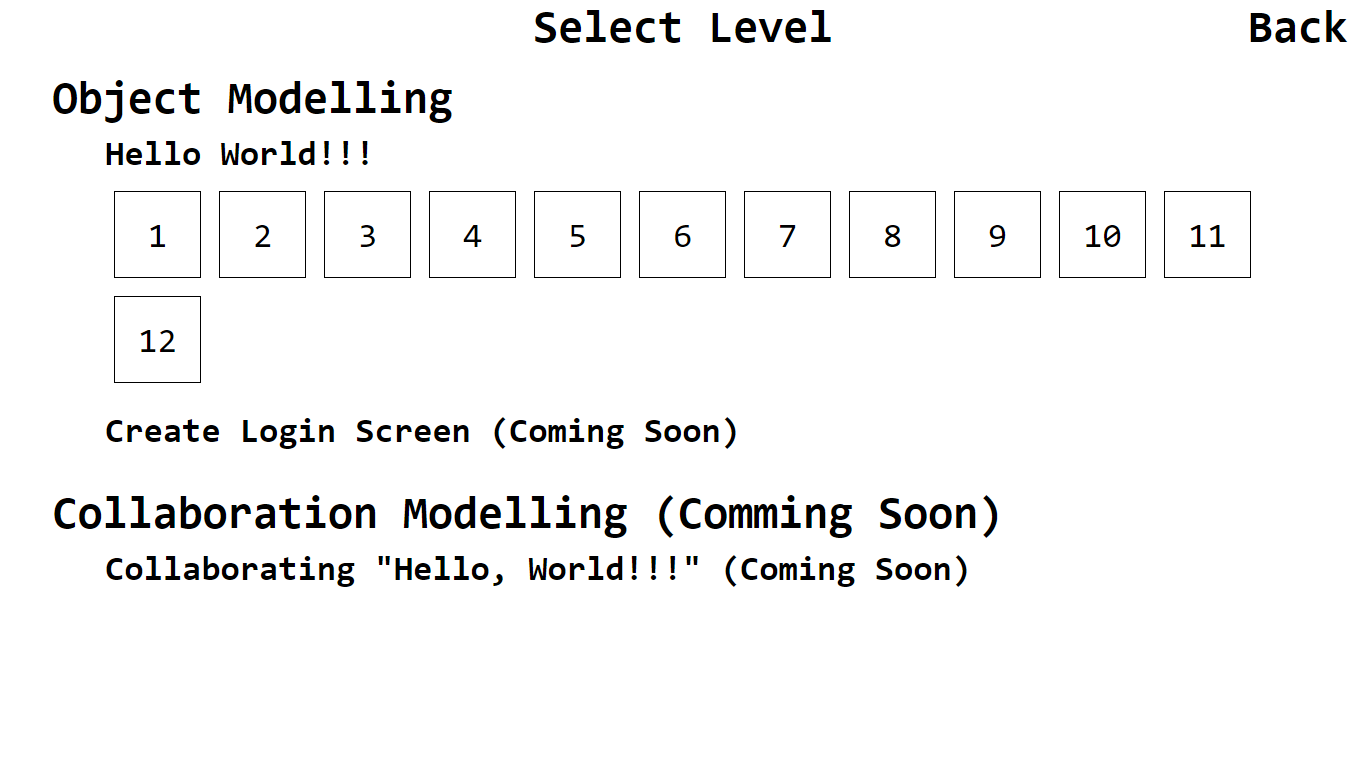
\includegraphics[height=3.5cm]{levels}}}
\hspace*{\fill}
\subfloat[Positive Reinforcement]{\frame{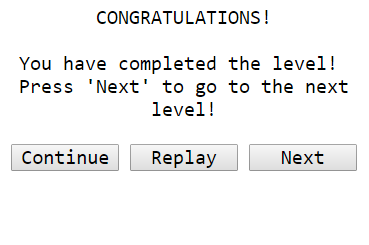
\includegraphics[height=3.5cm]{positive}}}
\caption{Game and learning elements embedded into the artifact.}
\end{figure}

\begin{figure}[htb]
\centering
\frame{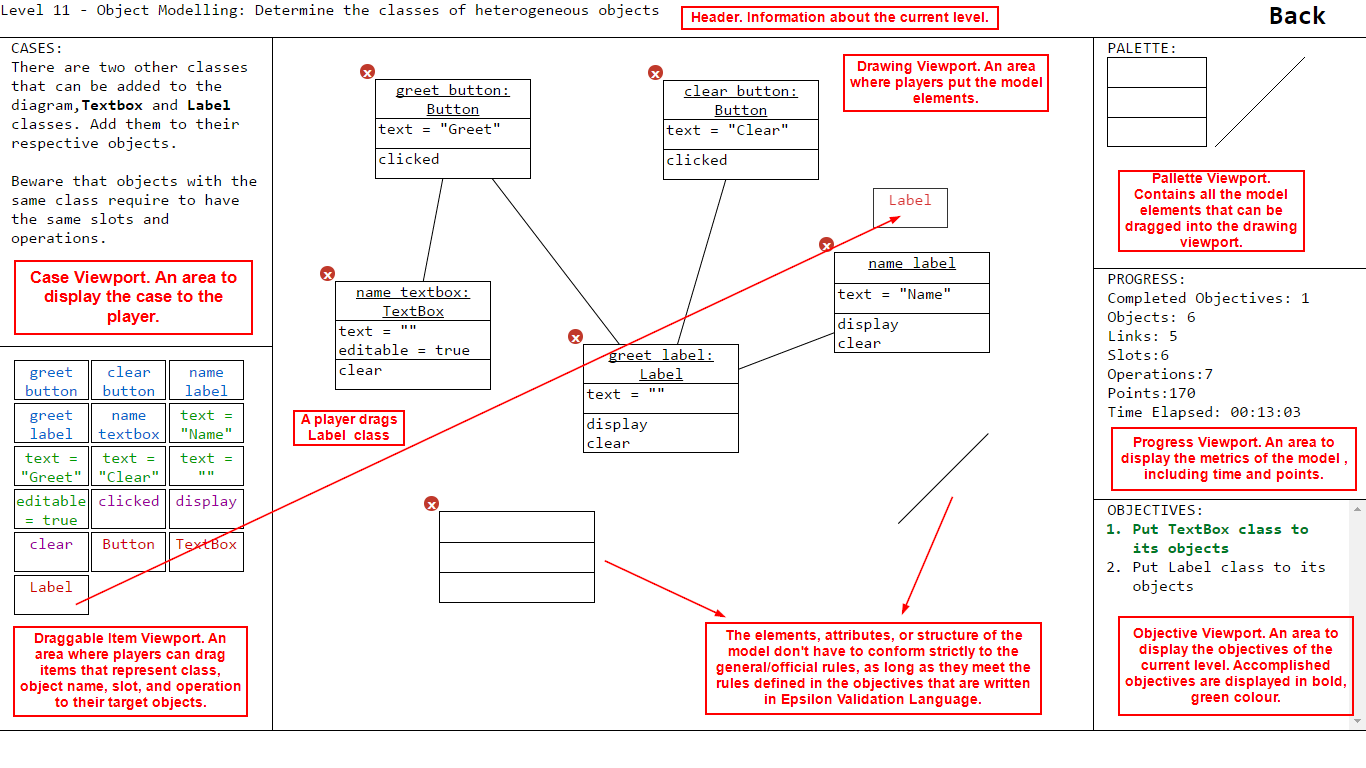
\includegraphics[width=\textwidth]{game-annotated}}
\caption{The game's display.}
\end{figure}

\subsection{Architecture}

\subsection{Model Validation}

\subsection{Modelling Editor}

\begin{figure}[htb]
\centering
\frame{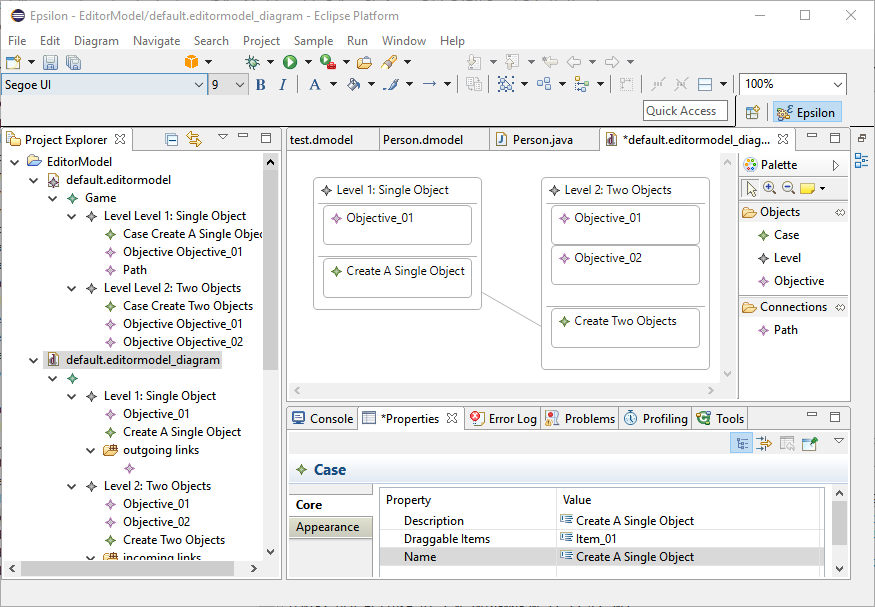
\includegraphics[width=\textwidth]{editor}}
\caption{Game editor to automatically generate the game.}
\end{figure}


\section{Conclusion}
 

\subsubsection*{Acknowledgments.} We would like to thank our respondents that participated in our preliminary interview. This research is supported by \emph{Lembaga Pengelola Dana Pendidikan Indonesia} (Indonesia Endowment Fund for Education). 

\bibliography{references} 
\bibliographystyle{ieeetr}

\end{document}

